%DO NOT MESS AROUND WITH THE CODE ON THIS PAGE UNLESS YOU %REALLY KNOW WHAT YOU ARE DOING
\chapter*{Modelling the Project}
\addcontentsline{toc}{chapter}{Modelling the Project}
\noindent It can be easy to lose sight of the core elements that make up any project. Each of these elements ties into the others, and together, they form the fabric that is this project. The prime four elements in the project are the tasks, the resources, the interested parties and the environment. The composition of each of these elements is shown in Figure 1 and is also discussed in the next topic.

\begin{figure}[H]
\centering
{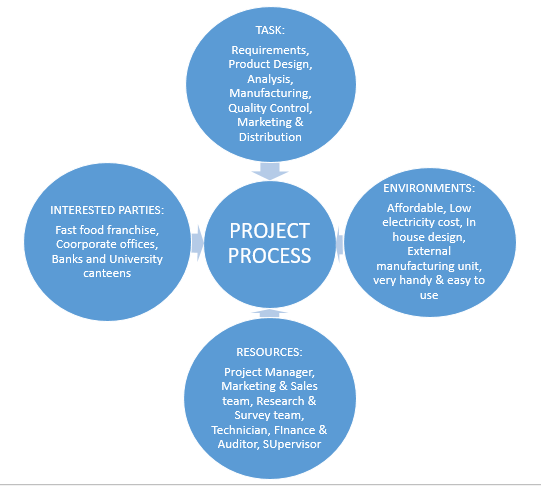
\includegraphics[scale=0.8]{basic.png}}
\caption{Basic Elements of a Project}
\end{figure}

\section{ The Tasks } \label{ The Tasks }
\noindent The task in this project is to cater to the specific requirement of the consumer especially for home use  with the intention of providing the consumer with the option of selecting the types of coffee grind size he/she wants and also providing them good quality powder with an easy to use mechanism thereby moving a step further of the machines which are available in the market for home use/offices/colleges/food franchise. The tasks comprises of research on what is required in-order to develop the coffee grinder, product design, analysis, manufacturing, quality control, marketing and distribution.

\section{ The Resources } \label{ The Resources }
\noindent The resources cover a very wide range. They include knowledge, ability, people, buildings, machines, money, etc. The main resources are the teams that are assigned for the specific tasks.

\section{ The Interested Parties } \label{ The Interested Parties }
\noindent If you understand the needs, expectations, and requirements of your interested parties, it is easy to see that these are critical to ensuring that your products or services meet requirements. So, it is important to know and understand your interested parties if you are to properly plan and implement the processes of your project. Without doing this critical step well, you run the risk of having problems when your product or service is used.

\noindent Offices, canteens and Banks comprise of many individuals having different taste buds and thus prefer to have various types of coffees. Hence it is always better to have a coffee grinder which could grind in various sizes in-order to have different types of coffees depending on ones mood. Fast food franchise would find the coffee grinder a simple and faster tool to cater the needs of many customers. Positively interested parties are ready to contribute to this by providing supporting arguments, feedback, or direct support in the form of cross marketing or other resources. The negatively interested parties would be the competitors, companies selling pre-ground coffee and the health ministry. Compliance obligations might include all relevant legal requirements, all requirements imposed by upper levels in the organisation (for example corporate requirements) and all relevant requirements of relevant interested parties that the organisation decides to comply with, whether contractually (customers) or voluntarily (environmental or safety commitments).

\section{ The Environment } \label{ The Environment }
\noindent The project environment artefacts evolve through three discrete states: the prototyping environment, the development environment, and the maintenance environment. The prototyping environment includes an architecture testbed for prototyping project architectures to evaluate trade-offs during the inception and elaboration phases of the life cycle. The development environment should include a full suite of development tools needed to support the various process workflows and to support round-trip engineering to the maximum extent possible. The maintenance environment should typically coincide with a mature version of the development environment. In some cases, the maintenance environment may be a subset of the development environment delivered as one of the project's end products.